\documentclass{article}

\usepackage{neurips_2019_author_response}

\usepackage[utf8]{inputenc} % allow utf-8 input
\usepackage[T1]{fontenc}    % use 8-bit T1 fonts
\usepackage{hyperref}       % hyperlinks
\usepackage{url}            % simple URL typesetting
\usepackage{booktabs}       % professional-quality tables
\usepackage{amsfonts}       % blackboard math symbols
\usepackage{nicefrac}       % compact symbols for 1/2, etc.
\usepackage{microtype}      % microtypography
\usepackage{xcolor}

\usepackage{graphicx}
\usepackage{amsmath,amssymb}
\usepackage{amsthm}
\newtheorem{thm}{Theorem}[section]
\usepackage{lipsum}
\usepackage{bm}

\input macros.tex

\begin{document}
We thank the reviewers for the helpful comments and feedback. Our responses are detailed below.

{\bf To Reviewer 1.} 
\vspace{-.15cm}

- In the description of Table 1:  $\bar \lambda$ is the sparsity penalty parameter averaged across $50$ simulations. 
%We realize that the original definition of $\bar \lambda$  (in the legend of Table 1) may cause confusion, and we will add the explanation to the main text. 

- Wording in L59, L131, L230. We will make the suggested edits for clarity. 

- Sparsity experiment and Table 1. We will remove the baseline case ($\lambda=0$) from Table 1. The ``sparsity $\rho$'' in the description should be corrected to ``sparsity ($p$)''. 

- Real data: %we agree with the  that adding numerical summaries to real data analysis will strengthen the paper. 
We will add the following additional analysis to the Section \emph{7.3.\ real data}. Specifically, we ran the clustering analysis on the \emph{Brain expression} and \emph{Nations} datasets and then compared the goodness-of-fit of different methods. Because the code of CoCo method [Chi et al, 2018] is not yet available as of 07/31/2019, we excluded it from our numerical comparison (we did have a theoretical comparison with CoCo). The following table summarizes the proportion of variance explained by each clustering method:
\vspace{-.15cm}
\begin{center}
\caption{Table: Comparison of goodness-of-fit in the \emph{Brain} expression and \emph{Nations} datasets.}
\begin{tabular}{c|cccccc}
Dataset& {\color{red}TBM} & {\color{red}TBM-sparse}&  CP&Tucker & CoTeC [Jegelka et al 2009]&CoCo [Chi et al 2018]\\
\hline
Brain expression&{\color{red}0.856}&{\color{red}0.855}&0.576&0.434&0.849&-\\
Nations&{\color{red}0.439}&{\color{red}0.433}&0.324&0.253&0.419&-\\
\end{tabular}
\end{center}
\vspace{-.15cm}
Our method (TBM) achieves the highest variance proportion, suggesting that the entries within the same cluster are close (i.e., a good clustering). As expected, the sparse TBM results in a slightly lower proportion, because it has a lower model complexity at the cost of small bias. It is remarkable that the sparse TBM still achieves a higher goodness-of-fit than others. The improved interpretability with little loss of accuracy makes the sparse TBM appealing in applications. 

{\bf To Reviewer 2.}
\vspace{-.15cm}

- Measuring MSE in a clustering problem. We agree with reviewer that MSE is not the best metric for clustering. In fact, Theorem 2 of our paper provides a consistency result for mis-classification rate (MCR) specifically for clustering. In addition, we also compared the empirical clustering error rate (CER, i.e., 1 - rank index) in the simulation. Both metrics, combined with the MSE, provided a fair comparison in the clustering problem. 
Following the reviewer's suggestion, we now upgrade the consistency result to a finite-sample convergence rate and will add the result below to the final paper.  
%\vspace{-.05cm}
%For membership matrix $\mM_k\in\{0,1\}^{R_k\times d_k}$, define the cluster proportion vector $\mp_k={1\over d_k}\mM_k\mathbf{1}_k$, where $\mathbf{1}_k$ is a length-$d_k$ vector with every entry to be 1. 
\begin{thm} [Simplified version]
Consider a Gaussian tensor block model with variance parameter $\sigma^2$ and non-degenerate clusterings. In the case when $d_1=\ldots=d_K=d$ and $R_1=\ldots=R_K=R$, we have
\vspace{-.05cm}
\[
\mathbb{P}(MCR(\hat \mM_k,\mP_k\mM_{k,\text{true}})\geq \varepsilon)\leq 2R^{K(d+1)} \exp\left( - {C_2  \delta_{\min}^2  d^K\varepsilon^2\over \sigma^2 }
\right),\quad \text{for all }k\in[K],
\]
\vspace{-.4cm}

where $\mP_k\in\mathbb{R}^{R_k\times R_k}$ is a permutation matrix, $C_2>0$ is a constant independent of tensor dimension, and $\delta_{\min}>0$ is the minimal gap (under some natural measurement) between tensor block means. 
\end{thm}
\vspace{-.3cm}
The above result implies that the clustering error converges to zero at the rate of $\tO({\sigma \over d^{(K-1)/2}\delta_{\min} })$. Here the block-mean gap $\delta_{\min}$ serves the role of the eigen-separation as in classical tensor Tucker decomposition. 
%Note that our method allows diminishing gap as $d\to \infty$, as long as $\delta\gg  d^{-(k-1)}$. 

- Data experiments. Regarding the real data, please see our response to Reviewer 1. Regarding the toy data, we have added the suggested numbers of clusters. See the figure below. The added curves now fill in the gap in the figure. 
\vspace{-.15cm}
\begin{center}
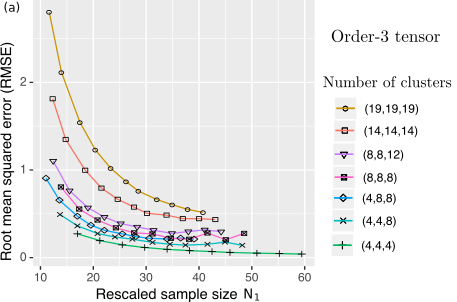
\includegraphics[width=4.7cm]{figure.pdf}
\hspace{.6cm}
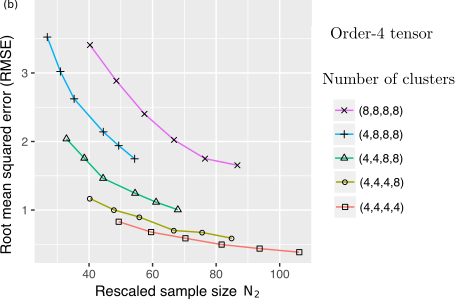
\includegraphics[width=5.3cm]{rescale_order4.pdf}
\end{center}
\vspace{-.6cm}
%- Real data experiments. Please see our response to (1). 

{\bf To Reviewer 3.}
\vspace{-.15cm}

- Novelty. Our method is related to, but also clearly distinctive from, previous methods in three aspects: accuracy, interpretability, and scalability.  The table below summarizes the comparison. In practice, our TBM method performs favorably in both simulation and real data (see our newly added analysis in response to Reviewer 1). Since tensor-valued data is now common in a number of fields, we believe this work will be of interest to the community. 

\vspace{-.1cm}
\resizebox{\columnwidth}{!}{
\begin{tabular}{c|ccc|c}
Method&Recovery error (MSE) & Clustering error (MCR)& Block detection& Time complexity (flop / iter)\\
\hline
Tucker (rigorous; $K=3$) & $dR$&${\sigma \over d\lambda_{\min}}$ up to rotation& No&$d^K$ \\
CoCo [Chi et al 2018] (rigorous) &$d^{K-1}$&-&No& $d^{K+1}$ or $d^K$\\
{\color{red}TBM (rigorous, this paper)} &{\color{red}$d\log R$}& {\color{red}$ {\sigma \over d^{(K-1)/2}\delta_{\min}}$}&{\color{red}Yes}&{\color{red}$d^K$}\\
Optimal rate [Gao et al 2018] (heuristic)& $d\log R$&-&-&-
\end{tabular}
}
\vspace{-.15cm}

-- Regarding the equation numbers in the Supplement, we will correct them in the final version. 

\end{document}